\documentclass[../../lecture_notes.tex]{subfiles}
\begin{document}


10. Scheduling Policies

We use the following processes to compare scheduling policies:
\begin{center}
\begin{tabular}{ | c | c | c | }
	\hline
	Jobs & Arrival Time & Work \\
	\hline\hline
	A & 0 & 3 \\
	\hline
	B & 1 & 5 \\
	\hline
	C & 3 & 2 \\
	\hline
\end{tabular}
\end{center}


We denote the cost of a context switch as "$\delta$".

\subsubsection*{FIRST-COME, FIRST-SERVED (FLFS)}
The process:
	\begin{enumerate}
	\item hold a queue of threads waiting to run
	\item run threads to completion
	\end{enumerate}
This is good for batch application with pre-known tasks (payroll, auditing, etc.)

\begin{minipage}{0.5\linewidth}
\[ \begin{array} { c | c | c }
	\text{Jobs} & \text{Wait Time} & \text{Turnaround Time} \\
	\hline
	A & 0 & 5 \\
	B & 4 + \delta & 6 + \delta \\
	C & 5 + 2\delta & 14 + 2\delta \\
	D & 13 + 3\delta & 17 + 3\delta \\
	\text{AVG} & 5.5 + 1.5\delta & 10.5 + 1.5\delta
\end{array} \]
\end{minipage}%
\begin{minipage}{0.5\linewidth}
\begin{tikzpicture}
\begin{axis}[ 
	axis x line*=center, axis y line=none, xtick={0,3,8,10}, axis equal, xmin=0, xmax=10
]
\addplot[mark=none] (1.5, 0.5) node {A};
\addplot[mark=none] (5.5, 0.5) node {B};
\addplot[mark=none] (9, 0.5) node {C};
\end{axis}
\end{tikzpicture}

Properties:
\begin{enumerate}[nosep]
\item[+] fair
\item[+] utilization
\item[-]  long wait time
\item[-] convoy effect
\end{enumerate}
\end{minipage}

Total time of execution = $20 + 3\delta$

*  the cost of a context switch is cheap here, since no save state is necessary


\subsubsection*{SHORTEST JOB FIRST (SJF)}
The process:
	\begin{enumerate}[nosep]
	\item hold a min-heap of waiting threads
	\item run threads to completion
	\end{enumerate}
This algorithm makes the assumption that runtimes are (roughly) known.

\begin{minipage}{0.5\linewidth}
\[ \begin{array}{ c | c | c }
	\text{Jobs} & \text{Wait Time} & \text{Turnaround Time} \\
	\hline
	A & 0 & 5 \\
	B & 4 + \delta& 6 + \delta \\
	C & 9 + 3\delta & 18 + 3\delta \\
	D & 4 + 2\delta & 8 + 3\delta \\
	\text{AVG} & 4.25 + 1.5\delta & 9.25 + 1.5\delta
\end{array} \]
\end{minipage}%
\begin{minipage}{0.5\linewidth}
\begin{center}
\begin{tikzpicture}
\begin{axis}[ 
	axis x line*=center, axis y line=none, xtick={0,3,5,10}, axis equal, xmin=0, xmax=10
]
\addplot[mark=none] (1.5, 0.5) node {A};
\addplot[mark=none] (4, 0.5) node {C};
\addplot[mark=none] (7.5, 0.5) node {B};
\end{axis}
\end{tikzpicture}
\end{center}

Properties:
\begin{enumerate}[nosep]
\item[+] improved avg weight and turnaround time
\item[+] high utilization
\item[-] unfair: starvation
\end{enumerate}
\end{minipage}

Total time of execution = $20 + 3\delta$

*  the cost of a context switch is cheap here, since no save state is necessary


\subsubsection*{ROUND-ROBIN (RR)}
The process: FCFS, but each process is only run for a set time slice

This algorithm necessitates preemption.

\begin{minipage}{0.5\linewidth}
\[ \begin{array}{ c | c | c }
	\text{Jobs} & \text{Wait Time} & \text{Turnaround Time} \\
	\hline
	A & 0 & 15 + 14\delta \\
	B & \delta & 5 + 5\delta \\
	C & 2\delta & 18 + 15\delta \\
	D & 3\delta & 11 + 13\delta \\
	\text{AVG} & 4.25 + 1.5\delta & 12.25 + 11.25\delta
\end{array} \]
\end{minipage}%
\begin{minipage}{0.5\linewidth}
\begin{center}
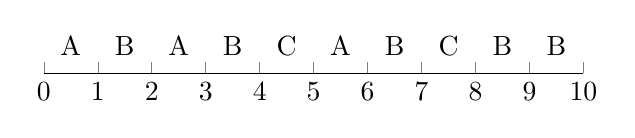
\begin{tikzpicture}
\begin{axis}[ 
	axis x line*=center, axis y line=none, xtick={0,1,2,3,4,5,6,7,8,9,10}, axis equal, xmin=0, xmax=10
]
\addplot[mark=none] (0.5, 0.5) node {A};
\addplot[mark=none] (1.5, 0.5) node {B};
\addplot[mark=none] (2.5, 0.5) node {A};
\addplot[mark=none] (3.5, 0.5) node {B};
\addplot[mark=none] (4.5, 0.5) node {C};
\addplot[mark=none] (5.5, 0.5) node {A};
\addplot[mark=none] (6.5, 0.5) node {B};
\addplot[mark=none] (7.5, 0.5) node {C};
\addplot[mark=none] (8.5, 0.5) node {B};
\addplot[mark=none] (9.5, 0.5) node {B};
\end{axis}
\end{tikzpicture}
\end{center}
Properties
\begin{enumerate}[nosep]
\item[+] fair, if new jobs are placed at the end of the queue (pictured algorithm does not do that)
\item[+] shorter wait time
\item[-] lower utilization
\end{enumerate}
\end{minipage}

Total time of execution = $20 + 15\delta$

*  the total time to run all of the tasks has gone up

The above scheduling policies have been static, some scheduling policies are dynamic, and depend on the state of the environment of the machine.


\subsubsection*{PRIORITY SCHEDULING}
The process: Jobs are given priority, and the highest runs first

Linux uses an inverted version with “niceness”, where nice tasks will defer to others. Students can increase niceness, but not lower it
\begin{lstlisting}
nice.c = {
	read args
	set priority
	execvp("gcc", (char* []){"gcc", "foo.c");
}
\end{lstlisting}

Specifically, this is an example of dynamically assigned priority

There is an even more complicated version of this called a:
\subsubsection*{MULTILEVEL FEEDBACK QUEUE (MLFQ)}
Goals:
	\begin{enumerate}[nosep]
	\item optimize turnaround time
	\item responsive to interactive users
	\item optimize response time
	\end{enumerate}
Maintain many queues with distinct priority levels.

The process: Round Robin within a queue according to the rules:
\begin{enumerate}[label=(\roman*), nosep]
	\item if P(A) > P(B), run A
	\item If P(A) = P(B), Round Robin
	\item new jobs enter at top queue
	\item jobs move down a queue after using time allotment
	\item boost all jobs to the top queue after a set time interval
\end{enumerate}

Parametrizing the time interval is tough; it is a voodoo constant. Some find this value using \term{decay-usage algorithms}. Others let users manipulate it with hints, called advice.


\end{document}